\documentclass[11pt]{article}

\usepackage{amsmath}
\usepackage{amssymb}
\usepackage[margin=0.68in]{geometry}
\usepackage{booktabs}
\usepackage[american]{circuitikz}
\usepackage{enumitem}
\usepackage{fancyhdr}
\usepackage{graphicx}
\usepackage[table]{xcolor}
\usepackage[hidelinks]{hyperref}
\usepackage{listings}
\usepackage{microtype}
\usepackage{tabularx}
\usepackage{tikz}
\usepackage{titlesec}
\usetikzlibrary{arrows.meta,positioning}
\graphicspath{{docs/lessons/assets/}{../assets/}}

\definecolor{AdkBlue}{gray}{0}
\definecolor{AdkRed}{gray}{0}
\definecolor{AdkGreen}{gray}{0.20}
\definecolor{CodeGray}{gray}{0.96}
\hypersetup
{
    pdftitle={ADK Lesson 009: Adaptive Night Light},
    pdfauthor={Kevin Shanahan},
    pdfsubject={Deterministic analog sensing, filtering, hysteresis, fault diagnosis, and PWM project},
    pdflang={en-US}
}
\pagestyle{fancy}
\fancyhf{}
\lhead{\textsc{ADK Lesson 009}}
\rhead{Adaptive Night Light}
\cfoot{\thepage}
\setlength{\headheight}{14pt}
\setlength{\parindent}{0pt}
\setlength{\parskip}{5pt}
\setlist{nosep,leftmargin=1.45em}
\titleformat{\section}{\Large\bfseries\color{AdkBlue}}{\thesection}{0.5em}{}
\titleformat{\subsection}{\large\bfseries\color{AdkBlue}}{\thesubsection}{0.5em}{}
\lstdefinestyle{adkcpp}
{
    language=C++,
    backgroundcolor=\color{CodeGray},
    basicstyle=\ttfamily\small,
    keywordstyle=\color{AdkBlue}\bfseries,
    commentstyle=\color{AdkGreen},
    columns=fullflexible,
    keepspaces=true,
    showstringspaces=false,
    frame=single,
    rulecolor=\color{black!20},
    breaklines=true,
    tabsize=4
}
\newcommand{\checkbox}{\(\square\)}
\newcommand{\blank}[1]{\rule{#1}{0.4pt}}
\newcommand{\warningbox}[1]{%
  \begin{center}
  \fcolorbox{AdkRed}{AdkRed!6}{\parbox{0.91\linewidth}{\textbf{\color{AdkRed}Safety checkpoint.} #1}}
  \end{center}}
\newcommand{\evidencebox}[1]{%
  \begin{center}
  \fcolorbox{AdkBlue}{AdkBlue!5}{\parbox{0.91\linewidth}{#1}}
  \end{center}}

\begin{document}

\begin{center}
  {\Huge\bfseries Adaptive Night Light}\\[4pt]
  {\Large Measure, decide, illuminate, and explain why}\\[8pt]
  \textit{The circuit makes its internal decision visible without requiring Serial.}
\end{center}

\begin{tabularx}{\linewidth}{@{}>{\bfseries}l X >{\bfseries}l X@{}}
Lesson & 009 --- integration project & Time & 150--210 minutes\\
Prerequisites & Lessons 001--008 & Board & Arduino Mega 2560\\
Evidence & voltage, raw sample, mode, PWM & Status & host verified; bench open\\
Safety & E1: USB-powered passive sensor and current-limited LEDs only\\
\end{tabularx}

\section{Mission and evidence chain}

Build a night light whose behavior can be explained at every layer:
\[
\text{ambient light}\rightarrow
\text{A0 voltage}\rightarrow
\text{raw sample}\rightarrow
\text{filtered permille}\rightarrow
\text{hysteresis mode}\rightarrow
\text{D9 PWM}.
\]
The white lamp is the primary output. A common-cathode RGB LED is the diagnostic
output: blue means \texttt{Ready}, green means \texttt{Active}, and red means
\texttt{SensorFault}. The named sensor test point is the divider junction at
A0; the named safe-state test point is D9 relative to GND.

By the end, you can:

\begin{itemize}
  \item compose \texttt{AnalogInput}, calibration, moving average, deadband,
        \texttt{NightLight}, \texttt{PwmOutput}, and \texttt{RgbLed};
  \item explain why calibration, filtering, deadband, and hysteresis solve
        different problems;
  \item reproduce a decision from an ordered sample trace;
  \item distinguish sensor open/short evidence from ordinary darkness or light;
  \item prove resource acquisition separately from the lamp's safe state;
  \item build, upload, monitor, and capture optional logs entirely from the CLI.
\end{itemize}

\warningbox{Disconnect USB and all other power before wiring. Use one
330\(\Omega\) resistor for the white LED and one for each RGB die. The sensor
divider must remain between the Mega's 5\,V and GND rails; never apply an
external signal to A0. Stop for heat, odor, resets, flicker unrelated to the
lesson, or any measured voltage outside 0--5\,V.}

\section{System composition}

\begin{center}
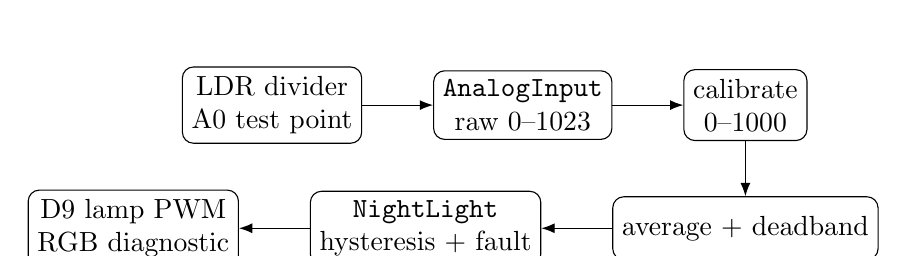
\begin{tikzpicture}[
    node distance=7mm and 9mm,
    box/.style={draw,rounded corners,minimum height=8mm,align=center},
    >=Latex]
  \node[box] (sensor) {LDR divider\\A0 test point};
  \node[box,right=of sensor] (analog) {\texttt{AnalogInput}\\raw 0--1023};
  \node[box,right=of analog] (cal) {calibrate\\0--1000};
  \node[box,below=of cal] (filter) {average + deadband};
  \node[box,left=of filter] (logic) {\texttt{NightLight}\\hysteresis + fault};
  \node[box,left=of logic] (outputs) {D9 lamp PWM\\RGB diagnostic};
  \draw[->] (sensor) -- (analog);
  \draw[->] (analog) -- (cal);
  \draw[->] (cal) -- (filter);
  \draw[->] (filter) -- (logic);
  \draw[->] (logic) -- (outputs);
\end{tikzpicture}
\end{center}

The canonical sketch deliberately reads like this diagram. Its \texttt{loop()}
first calls \texttt{observeLight()}, then \texttt{decideLighting()}, then
\texttt{actuateLighting()}. Hardware ownership remains in the endpoints;
\texttt{NightLight} receives a value and knows nothing about Arduino pins.

\subsection{Why four transformations?}

\begin{tabularx}{\linewidth}{@{}l X X@{}}
\toprule
Stage & Question answered & What it does not prove\\
\midrule
Calibration & What normalized light does this raw value represent? & Stability over time\\
Moving average & What recent level does a noisy stream support? & A mode decision\\
Deadband & Is this tiny change worth reporting? & Lamp on/off policy\\
Hysteresis & Has light crossed the appropriate boundary for the current mode? & Electrical output\\
\bottomrule
\end{tabularx}

\section{Authoritative pencil build plate}

\begin{figure}[ht]
  \centering
  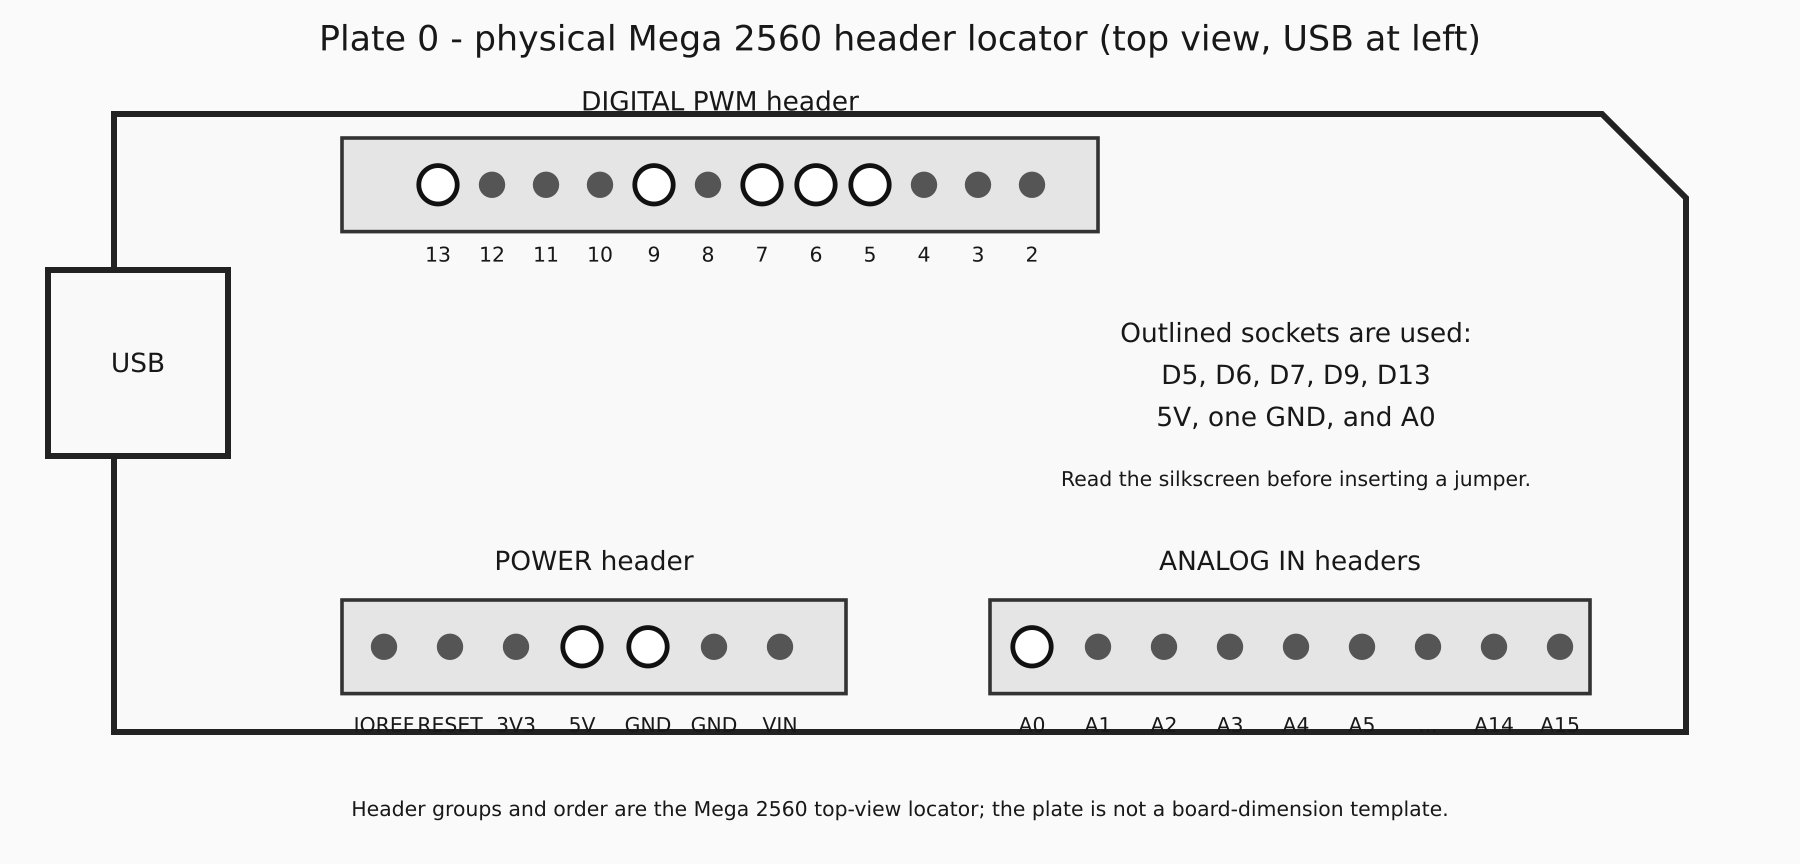
\includegraphics[width=\linewidth]{009-mega-header-locator.png}
  \caption{Plate 0 locates the used sockets in their physical Mega 2560 header
  groups and order. Orient the board with USB at left and still confirm the
  printed silkscreen before inserting a jumper.}
\end{figure}

\begin{figure}[ht]
  \centering
  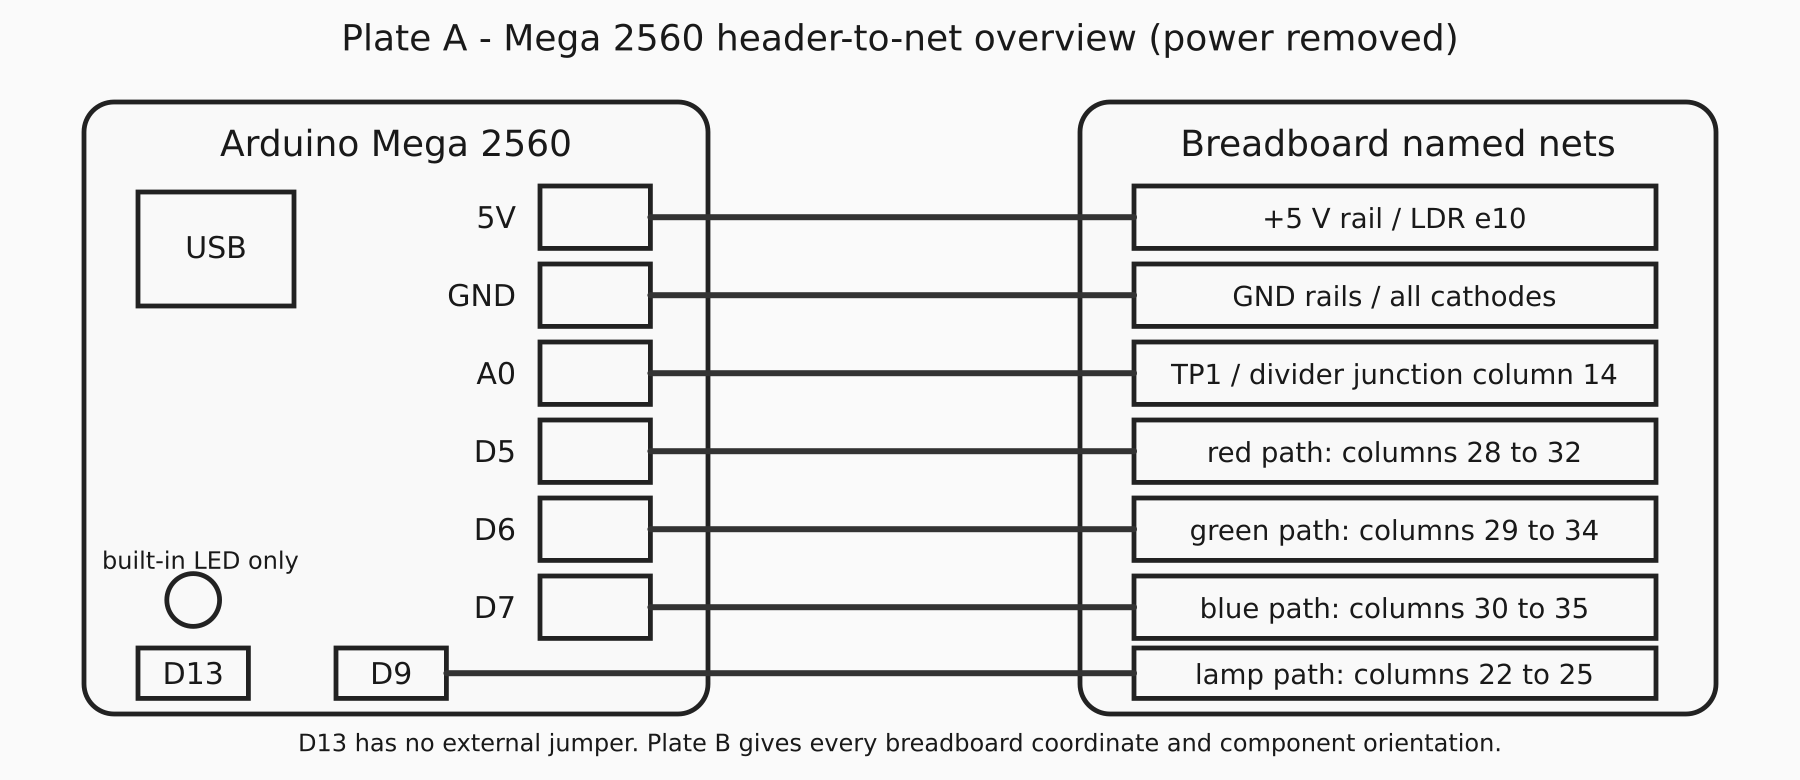
\includegraphics[width=\linewidth]{009-night-light-overview.png}
  \caption{Plate A separates every used physical Mega header from its named
  breadboard net. D13 is the built-in LED and has no external jumper.}
\end{figure}

\begin{figure}[ht]
  \centering
  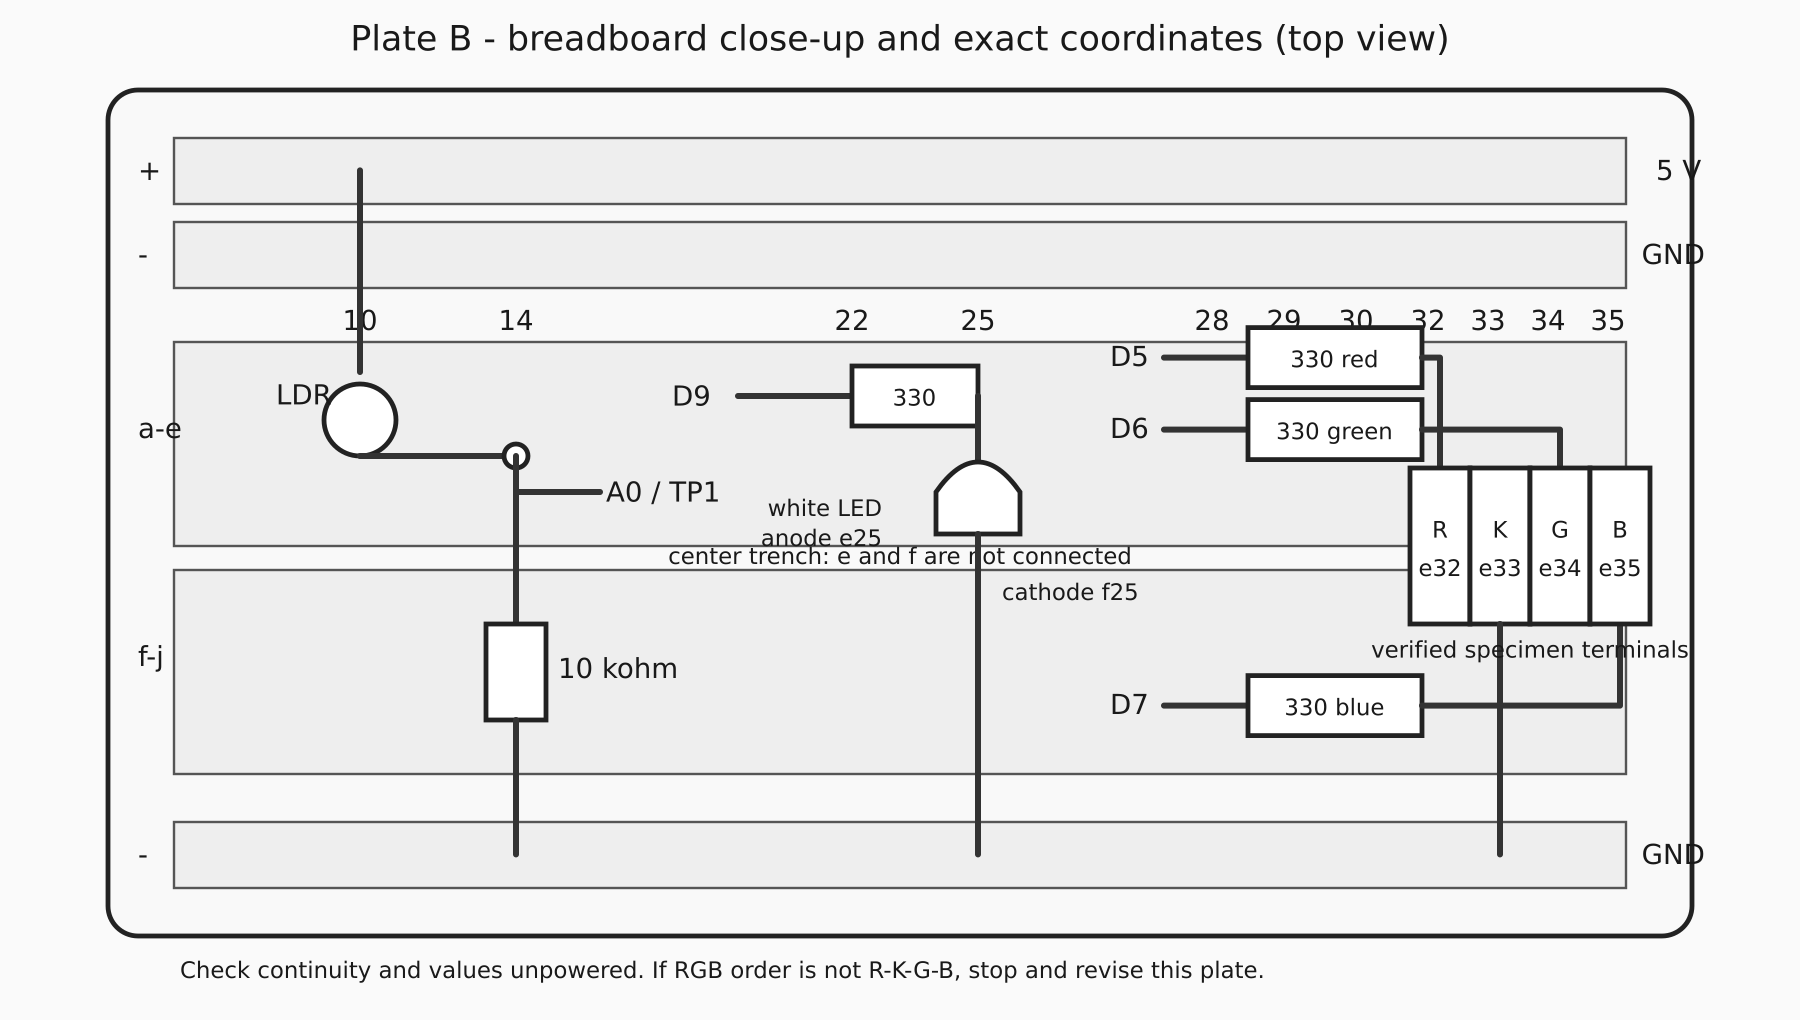
\includegraphics[width=\linewidth]{009-night-light-breadboard.png}
  \caption{Plate B enlarges breadboard topology, coordinates, polarity, and
  resistor placement. Cross-check both plates against the manifest below.}
\end{figure}

\section{Parts and literal wiring}

\begin{tabularx}{\linewidth}{@{}l l X@{}}
\toprule
Quantity & Part & Requirement\\
\midrule
1 & Mega 2560 & USB powered\\
1 & photoresistor & identified passive LDR; record its datasheet or kit reference\\
1 & resistor & 10\,k\(\Omega\), divider lower leg\\
1 & white LED & identified polarity and forward-voltage range\\
1 & common-cathode RGB LED & verify package pinout; lead order is not universal\\
4 & resistors & 330\(\Omega\), one per LED die\\
1 & multimeter & DC voltage and unpowered resistance/continuity\\
\bottomrule
\end{tabularx}

\textbf{Specimen gate.} The authorized Elegoo family listing proves that an
LDR, white LED, and RGB LED belong to the kit; it does not prove the selected
specimen's electrical identity. Before wiring, record the LDR package/photo and
measured dark/light resistance; white LED package, anode/cathode, and
\(V_f\); and RGB package/photo, viewing orientation, individual lead numbers,
common-cathode lead, each color lead, and each color's \(V_f\). The build plate
uses the verified left-to-right RGB order R--K--G--B at e32--e35, viewed from
the flat/package reference recorded on the card. If the specimen differs,
stop: revise both the build plate and manifest before applying USB power.

\textbf{Coordinate net manifest.} The breadboard's a--e holes in one numbered
column are connected; f--j form a separate group across the center trench.
Power-rail breaks vary by board. Test continuity unpowered and add only the
rail bridge required for the used segment.

\begin{tabularx}{\linewidth}{@{}l X X@{}}
\toprule
Net & Exact build-plate path & Cross-check\\
\midrule
rails & Mega 5\,V to used top \(+\) rail; Mega GND to used top \(-\)
      rail; join used bottom \(-\) rail to the same GND & continuity to named
      Mega header; no 5\,V--GND continuity\\
sensor & \(+\) rail to LDR e10; other LDR lead e14; A0 to a14/TP1;
       10\,k\(\Omega\) from b14 to \(-\) rail & e14/a14/b14 are one junction;
       TP1 is measured only to GND\\
lamp & D9 to a22; 330\,\(\Omega\) e22--e25; white anode a25;
       white cathode f25 to bottom \(-\) rail & LED straddles trench; TP-LAMP
       is a25 to GND\\
RGB red & D5 to a28; 330\,\(\Omega\) e28--e32; verified red lead e32 &
       resistor measured unpowered\\
RGB return & verified common cathode e33 to bottom \(-\) rail & continuity to
       Mega GND\\
RGB green & D6 to b29; 330\,\(\Omega\) d29--d34; verified green lead e34 &
       resistor measured unpowered\\
RGB blue & D7 to c30; 330\,\(\Omega\) c30--c35; verified blue lead e35 &
       resistor measured unpowered\\
D13 evidence & Mega built-in LED only; no external breadboard jumper &
       250\,ms pulse, then 750\,ms dark separator\\
\bottomrule
\end{tabularx}

The fixed 10\,k\(\Omega\) lower leg limits divider current to at most
0.5\,mA at 5\,V even if the LDR is shorted. Its Thevenin source impedance is
never above 10\,k\(\Omega\), matching the conservative ADC source-impedance
guidance used in this lesson.

\begin{center}
\begin{circuitikz}[american voltages,scale=.85,transform shape]
  \draw (0,5) node[vcc]{5 V}
        to[phR,l={LDR}] (0,3)
        to[R,l={$10\,\mathrm{k}\Omega$}] (0,0) node[ground]{};
  \draw (0,3) to[short,*-o] (2.3,3)
        node[right,align=left]{A0 sensor test point\\measure to GND};

  \draw (5.0,4.4) node[left]{D9 PWM}
        to[short,o-] (5.7,4.4)
        to[R,l={$330\,\Omega$}] (7.7,4.4)
        to[leD,l={white lamp}] (9.7,4.4)
        -- (10.4,4.4) -- (10.4,3.8) node[ground]{};

  \foreach \y/\pin/\name in {2.7/5/red,1.7/6/green,0.7/7/blue}
  {
    \draw (5.0,\y) node[left]{D\pin}
          to[short,o-] (5.7,\y)
          to[R,l={$330\,\Omega$}] (7.7,\y)
          to[leD,l={RGB \name}] (9.7,\y) -- (10.4,\y);
  }
  \draw (10.4,.7) -- (10.4,2.7) -- (10.4,.1) node[ground]{};
\end{circuitikz}
\end{center}

More light lowers LDR resistance, raises A0 voltage, and raises the normalized
\texttt{lightPermille} value. If your identified sensor behaves differently,
change the divider orientation and calibration together; do not silently invert
only the software.

\subsection{Current and timer budget}

For each LED die, calculate \(I=(V_{OH}-V_f)/330\,\Omega\) with the actual
part's minimum \(V_f\) and a conservative loaded \(V_{OH}\). Record the
worst simultaneous case: the lamp plus up to three RGB dies. Keep margin below
every ATmega2560 pin, port-group, and package operating limit; absolute maximum
ratings are not design targets. This lesson additionally requires the calculated
and measured current to remain at or below 15\,mA per channel.

\begin{center}
\begin{tabularx}{\linewidth}{@{}l X X X@{}}
\toprule
Channel & measured \(V_f\) & calculated worst current & measured active current\\
\midrule
white / D9 & & &\\
red / D5 & & &\\
green / D6 & & &\\
blue / D7 & & &\\
\bottomrule
\end{tabularx}
\end{center}

Worst simultaneous case named: \blank{1.5in}. Calculated total:
\blank{.7in}\,mA. Measured total: \blank{.7in}\,mA. Record the actual
combination observed; do not add four single-channel measurements if the
firmware never commands that combination.

D9 uses the Mega's Timer2 PWM resource. D5, D6, and D7 use other PWM timers.
Do not add \texttt{PiezoSounder} without resolving its exclusive Timer2 claim:
the conflict must fail during initialization, before an active waveform.

\newpage
\section{Decision contract}

\begin{lstlisting}[style=adkcpp]
adk::NightLightConfig nightLightConfig;
nightLightConfig.turnOnBelowPermille  = 350;
nightLightConfig.turnOffAbovePermille = 450;
nightLightConfig.minimumDuty          = 24;
nightLightConfig.maximumDuty          = 192;

adk::NightLight nightLight (nightLightConfig);

const adk::NightLightInput observation (
    filteredLight,
    adk::LightSampleState::Valid);

nightLight.update (observation);
const adk::NightLightSnapshot decision = nightLight.snapshot ();
\end{lstlisting}

\texttt{NightLight} starts \texttt{Off}. After successful acquisition the
built-in D13 LED pulses for 250\,ms and stays dark for a 750\,ms separator;
normal behavior never drives it. A valid value strictly below 350
permille changes it to \texttt{On}; it remains on through the middle band and
changes off only strictly above 450. Equality does not cross either boundary.
This memory is hysteresis, not filtering.

\begin{center}
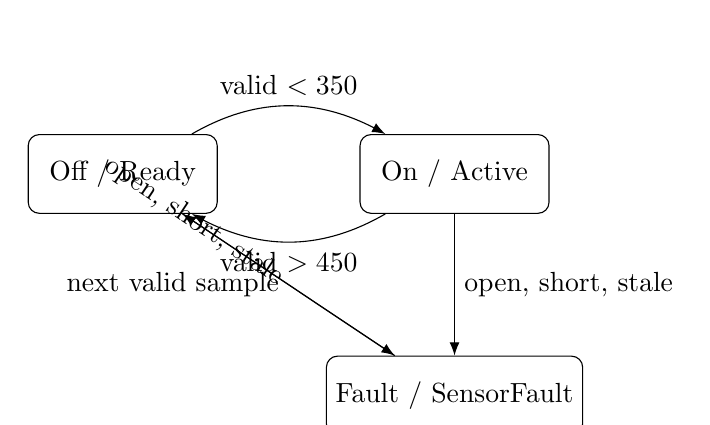
\begin{tikzpicture}[
    node distance=18mm,
    state/.style={draw,rounded corners,minimum width=24mm,minimum height=10mm},
    >=Latex]
  \node[state] (off) {Off / Ready};
  \node[state,right=of off] (on) {On / Active};
  \node[state,below=of on] (fault) {Fault / SensorFault};
  \draw[->,bend left] (off) to node[above]{valid \(<350\)} (on);
  \draw[->,bend left] (on) to node[below]{valid \(>450\)} (off);
  \draw[->] (off) -- node[left,sloped]{open, short, stale} (fault);
  \draw[->] (on) -- node[right]{open, short, stale} (fault);
  \draw[->] (fault) -- node[left]{next valid sample} (off);
\end{tikzpicture}
\end{center}

Any explicit \texttt{BelowRange}, \texttt{AboveRange}, or \texttt{Stale}
sample enters \texttt{Fault}, forces duty zero, and selects the red diagnostic.
The next valid sample first recovers to \texttt{Off}; darkness must then satisfy
the ordinary turn-on rule. This prevents a recovered sensor from inheriting an
old active command.

\section{Deterministic trace exercise}

Use an eight-sample moving average and an eight-permille deadband. For this
short worksheet, the ``filtered'' column is supplied so the state-machine
reasoning remains visible.

\begin{center}
\begin{tabular}{@{}rrrrllr@{}}
\toprule
Step & raw & filtered & state & prior mode & next mode & duty\\
\midrule
1 & 700 & 680 & Valid & Off & \blank{.55in} & \blank{.45in}\\
2 & 360 & 440 & Valid & Off & \blank{.55in} & \blank{.45in}\\
3 & 240 & 340 & Valid & Off & \blank{.55in} & \blank{.45in}\\
4 & 410 & 400 & Valid & On  & \blank{.55in} & \blank{.45in}\\
5 & 520 & 451 & Valid & On  & \blank{.55in} & \blank{.45in}\\
6 & 1023 & --- & AboveRange & Off & \blank{.55in} & \blank{.45in}\\
7 & 220 & 330 & Valid & Fault & \blank{.55in} & \blank{.45in}\\
\bottomrule
\end{tabular}
\end{center}

Replay the same ordered samples twice in the host test. Equal configuration and
samples must produce equal snapshots. No test reads wall time, sleeps, or
depends on Serial delivery.

\section{Fault matrix}

\begin{tabularx}{\linewidth}{@{}l X l l@{}}
\toprule
Fault or boundary & Expected decision & Lamp & RGB\\
\midrule
A0 near 0 & suspected divider fault; not ordinary darkness & duty 0 & red\\
A0 near 1023 & suspected divider fault; not ordinary daylight & duty 0 & red\\
missing fresh value & \texttt{Stale} & duty 0 & red\\
350 exactly while off & strict boundary does not turn on & duty 0 & blue\\
450 exactly while on & strict boundary does not turn off & active & green\\
D9 already claimed & initialization fails before operation & high impedance & unavailable or inactive\\
Timer2 exclusively claimed & initialization fails before PWM & high impedance & inactive\\
fixed 120\,s deadline & outputs inactive for 250\,ms, then reverse shutdown &
high impedance & high impedance\\
reset or shutdown & reset repeats acquisition; shutdown releases ownership &
high impedance & high impedance\\
\bottomrule
\end{tabularx}

\evidencebox{\textbf{Do not overclaim the RGB evidence.} Blue proves that all
objects initialized and the controller selected \texttt{Ready}. It does not
prove D9 is electrically safe. Measure D9 to GND separately: zero duty while
initialized should be near 0\,V. For high impedance, remove USB, install the
one-at-a-time 10\,k\(\Omega\)/10\,k\(\Omega\) midpoint fixture described below,
inspect it, restore USB, and measure the midpoint. Never use an ohmmeter on a
powered circuit.}

\section{CLI-only workflow}

No IDE is required. From the repository root:

\begin{lstlisting}[style=adkcpp,language=bash]
make bootstrap
make host-test
make arduino-Lesson009AdaptiveNightLight
arduino-cli compile --fqbn arduino:avr:mega --library . \
  --build-property \
  compiler.cpp.extra_flags=-DADK_LESSON009_ACCEPTANCE_TELEMETRY=1 \
  examples/Lesson009AdaptiveNightLight
make upload EXAMPLE=Lesson009AdaptiveNightLight PORT=/dev/ttyACM0
make monitor-describe PORT=/dev/ttyACM0
make monitor PORT=/dev/ttyACM0 BAUD=115200
make serial-log PORT=/dev/ttyACM0 BAUD=115200 \
    SERIAL_LOG=build/serial/lesson009.log
make lessons
make site
\end{lstlisting}

The circuit supplies the acceptance evidence even if \texttt{monitor} is never
run. The compile-time acceptance build emits only \texttt{raw=} ADC counts,
bounded to one record per 250\,ms and by the fixed 120\,s deadline. It is
supporting evidence for the TP1 voltage observation, never the acquisition or
safe-state proof. The default build has telemetry disabled.

\section{Bench procedure: predict, observe, interpret}

\subsection{Stage A --- inspect without power}

\begin{enumerate}
  \item \checkbox\ Confirm the exact Mega pins, every 330\(\Omega\) resistor,
        recorded RGB R--K--G--B specimen orientation, LDR divider orientation,
        and every build-plate coordinate.
  \item \checkbox\ Measure the divider's lower resistor:
        expected \(\blank{.7in}\), observed \(\blank{.8in}\).
  \item \checkbox\ Confirm no continuity from 5\,V directly to GND and no LED
        die lacks its series resistor.
  \item \checkbox\ Cross-check each manifest net with a second person or a
        second pass; mark every row only after continuity agrees.
  \item \checkbox\ Predict the A0 voltage in bright and covered conditions.
\end{enumerate}

\subsection{Stage B --- acquisition evidence}

Power from USB. Do not upload until the unpowered checks pass.

\begin{enumerate}
  \item \checkbox\ Build and upload with the CLI targets above.
  \item \checkbox\ Predict: D13 lights for 250\,ms, remains dark for the
        750\,ms separator, then valid moderate light selects blue.
  \item \checkbox\ Observe D13 timing: on \blank{.6in}\,ms; separator
        \blank{.6in}\,ms.
  \item \checkbox\ Observe RGB: \blank{1.7in}.
  \item \checkbox\ Interpret: \blank{4.4in}.
\end{enumerate}

\subsection{Stage C --- sensor and decision evidence}

\begin{enumerate}
  \item \checkbox\ Measure A0 to GND under bright light:
        predicted \blank{.55in}\,V / \blank{.55in} counts; observed
        \blank{.55in}\,V / \blank{.55in} counts. Cover the LDR:
        predicted \blank{.55in}\,V / \blank{.55in} counts; observed
        \blank{.55in}\,V / \blank{.55in} counts. Interpret whether count
        direction and measured rail ratio agree: \blank{2.0in}.
  \item \checkbox\ Move light slowly through the on boundary. Record A0 voltage
        when the lamp becomes active: \blank{.7in}\,V.
  \item \checkbox\ Reverse direction. Record voltage when it becomes ready:
        \blank{.7in}\,V. Explain the different boundaries:
        \blank{3.0in}.
  \item \checkbox\ Observe green with the lamp waveform. At D9, record PWM
        high level \blank{.6in}\,V; predicted duty \blank{.6in}\%;
        observed duty \blank{.6in}\%. Interpret: \blank{1.5in}.
\end{enumerate}

\subsection{Stage D --- fault and safe-state evidence}

Remove USB before changing the sensor connection. Simulate only one fault at a
time, then restore wiring unpowered.

\begin{enumerate}
  \item \checkbox\ With USB removed, move only the \(+\)-rail jumper from LDR
        e10 to an unused insulated row, leaving e14/a14/b14 and the 10\,k\(\Omega\)
        lower leg intact. Restore USB. Predict red and lamp duty zero.
        Observe: \blank{2.4in}.
  \item \checkbox\ Remove USB. Restore e10, then place one jumper e10--e14
        across only the LDR terminals. Inspect, restore USB, and predict red
        with duty zero.
        Observe: \blank{2.4in}.
  \item \checkbox\ Restore normal wiring. Confirm recovery goes through blue
        before darkness can select green.
  \item \checkbox\ Record D9 initialized at zero duty: \blank{.8in}\,V. Let the
        fixed 120\,s deadline expire. Observe lamp and RGB inactive for at
        least 250\,ms before release: \blank{1.5in}.
  \item \checkbox\ Remove USB. Disconnect the white LED/resistor path from D9.
        Install two 10\,k\(\Omega\) resistors in series from 5\,V to GND and
        connect their midpoint to D9 only. Inspect, restore USB, and after the
        fixed deadline record midpoint voltage \blank{.7in}\,V. A value near
        half the measured rail supports high impedance; near a rail does not.
        Remove USB before removing the fixture.
  \item \checkbox\ Repeat the midpoint test one output at a time for D5, D6,
        and D7, never with an LED path attached. Record:
        D5 \blank{.55in}\,V; D6 \blank{.55in}\,V; D7 \blank{.55in}\,V.
  \item \checkbox\ Press reset after restoring the normal circuit unpowered.
        Record the repeated D13 pulse/separator and Ready recovery:
        \blank{2.0in}.
\end{enumerate}

This procedure detects the named open and short simulations because the fixed
divider leg drives A0 toward a rail. A broken A0 jumper can float at a plausible
value and is not universally detectable with one ADC channel. Even then, every
accepted sample remains bounded and output duty cannot exceed the configured
maximum; inspect continuity unpowered when evidence disagrees.

\section{Diagnosis by layer}

\begin{tabularx}{\linewidth}{@{}l X X@{}}
\toprule
Observation & Most useful next check & Reason\\
\midrule
no RGB at startup & resource conflict, polarity, resistor, common cathode & acquisition evidence is absent\\
red RGB, lamp off & A0 voltage and divider continuity & controller reports sensor evidence invalid\\
blue/green changes, lamp dark & D9 waveform, LED polarity, lamp resistor & decision exists; actuator path is suspect\\
lamp chatters near threshold & raw range, average window, deadband, threshold order & separate noise from policy\\
A0 changes, mode does not & calibration direction and normalized values & electrical sensing works; mapping may not\\
unexpected reset & disconnect power and inspect shorts/current budget & software evidence cannot clear an electrical fault\\
\bottomrule
\end{tabularx}

\section{Design exercises}

\begin{enumerate}
  \item Plot measured A0 voltage against normalized permille at five light
        levels. Which calibration points should be learned from your room?
  \item Change only the moving-average window. Predict latency and noise before
        compiling; then record both.
  \item Change only the hysteresis gap. Find the smallest gap that avoids
        chatter in a repeatable hand-shadow trace.
  \item Propose a stale-sample policy using explicit time. State the maximum
        valid age and add rollover cases before changing the interface.
  \item Add a host trace for one sensor fault during active PWM. Prove the first
        fault snapshot commands zero duty and the first recovery snapshot is
        \texttt{Off}.
\end{enumerate}

\section{Acceptance record}

\begin{tabularx}{\linewidth}{@{}l X l X@{}}
\toprule
Field & Record & Field & Record\\
\midrule
Board/revision & & Date &\\
USB source/cable and measured 5\,V rail & & Reviewer &\\
Arduino CLI/core & & ADK revision &\\
Multimeter make/model/asset ID & & LDR package/photo/resistance &\\
Acceptance sketch artifact/hash & & Logic probe/scope make/model/asset ID &\\
White LED package/polarity/\(V_f\) & & RGB package/photo/R--K--G--B pin map &\\
Flash bytes & & Static RAM bytes &\\
\bottomrule
\end{tabularx}

\begin{itemize}
  \item \checkbox\ Unpowered wiring and current calculations passed.
  \item \checkbox\ Ready, Active, and SensorFault indications matched the table.
  \item \checkbox\ A0 voltage supported the raw-sample interpretation.
  \item \checkbox\ Hysteresis produced distinct on and off boundaries.
  \item \checkbox\ Open and short sensor tests forced lamp duty zero.
  \item \checkbox\ Resource acquisition and D9 safe state were proven separately.
  \item \checkbox\ Reset, shutdown, and power removal observations were recorded.
  \item \checkbox\ Measured rail, TP1 light extremes, each 330\,\(\Omega\)
        resistor, each active-channel current, and worst simultaneous current
        total were recorded.
\end{itemize}

Observed deviations and unresolved checks:
\vspace{0.45in}

\textbf{Release status.} Compilation, host replay, and a generated PDF do not
constitute physical verification. Until a person completes this card on the
named Mega 2560 and records measurements, this lesson remains host verified
with hardware acceptance open.

\section{Use with}

Use the maintained HTML lesson for searchable API links, errata, source
downloads, and exact CLI targets. Use this PDF at the bench for predictions,
schematics, worksheets, and recorded evidence. The canonical editable sketch
is \texttt{examples/Lesson009AdaptiveNightLight/} rather than a duplicate in
this document.

\begin{itemize}
  \item \href{https://spincyc.github.io/adk/lessons/009/}{Lesson 009 HTML}
  \item \href{https://github.com/spincyc/adk/tree/main/examples/Lesson009AdaptiveNightLight}{Canonical sketch}
  \item \href{https://github.com/spincyc/adk/blob/main/src/night_light.h}{NightLight API}
  \item \href{https://docs.arduino.cc/resources/datasheets/A000067-datasheet.pdf}{Arduino Mega 2560 datasheet}
  \item \href{https://www.microchip.com/en-us/product/ATmega2560}{ATmega2560 primary product page}
\end{itemize}

\end{document}
